\section{Mobile networks and security}

\question{Which vulnerability in the GSM network does the Stingray leverage?}
\begin{checkboxes}
    \CorrectChoice It exploits the fact that only the MS must authenticate in GSM.
    \choice It mounts a brute-force attack to recover the Ki and then decrypt all communications.
    \choice It uses the weaknesses in the A3/A8/A5 algorithms to mount a MITM attack.
    \choice It uses jamming to force a MS to connect to a rogue BS.
    \choice None of the other options.
\end{checkboxes}

\question{Which of the following are 2G vulnerabilities?}

\question{What are the main security issues in SS7 (Signaling System No. 7)?}
\begin{checkboxes}
    \CorrectChoice Caller ID spoofing and call redirection.
    \CorrectChoice Interception of SMS messages and phone calls.
    \choice Unauthorized access to subscriber billing information.
    \choice Location tracking of mobile devices.
    \choice None of the other options.
\end{checkboxes}

\question{Purpose of paging and location are in mobile network}

\question{What is the difference between the Visitor Location Register (VLR) and the Home Location Register (HLR) in GSM networks?}
\begin{checkboxes}
    \CorrectChoice The VLR is a temporary database that stores information about subscribers currently roaming in the coverage area, while the HLR is a permanent database that contains detailed subscriber information and is maintained by the subscriber's home network.
    \choice The VLR handles billing and account information for roaming subscribers, while the HLR manages encryption keys and authentication data.
    \choice The VLR is responsible for managing voice call routing, while the HLR handles data transmission services.
    \choice The VLR stores the IMSI and Ki keys, while the HLR stores the subscriber's phonebook and SMS messages.
    \choice None of the other options.
\end{checkboxes}


\question{Describe device authentication in GSM (completare l'immagine con le parti date.)}
\begin{solution}
    \center
    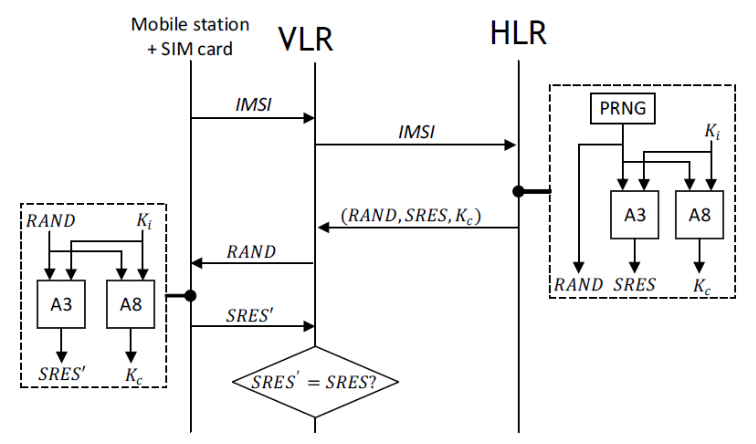
\includegraphics[width=0.7\textwidth]{images/GSM_auth.png}
\end{solution}


\question{4G networks - techniques used to enhance security}

\question{GSM Authentication}



\question{What is the primary purpose of handover in mobile networks?}
\begin{checkboxes}
    \choice To encrypt voice and data transmissions for secure communication.
    \choice To seamslessy transfer an active call or data session from one mobile teriminal to another.
    \choice To manage billing and account information for mobile subscribers when they move between to Base Stations.
    \choice To increase the data transmission speed betwen mobile devices.
    \CorrectChoice None of the other options.
\end{checkboxes}

\question{What are the main components involved in the GSM authentication process?}
\begin{checkboxes}
    \CorrectChoice SIM card, Authentication Center (AuC), and Home Location Register (HLR).
    \choice Mobile Equipment (ME), Visitor Location Register (VLR), and Base Transceiver Station (BTS).
    \choice Mobile Station (MS), Base Station Subsystem (BSS), and Network Switching Subsystem (NSS).
    \choice Mobile Management Entity (MME), Serving Gateway (SGW), and Packet Data Network Gateway (PGW).
    \choice None of the other options.
\end{checkboxes}

\question{What are the advantages and disadvantages of having small or larger cells in mobile networks?}
\begin{checkboxes}
    \choice Small cells are more expensive to deploy and maintain compared to larger cells, which are cheaper and more energy-efficient.
    \choice None of the other options.
    \choice Small cells are only suitable for urban areas, while larger cells can only be used in rural areas.
    \choice Small cells reduce interference and improve signal quality, whereas larger cells are prone to higher levels of interference and degraded signal quality.
    \CorrectChoice Small cells provide higher capacity and better coverage in dense areas but may require more frequent handovers as users move, while larger cells cover wider areas with fewer handovers but might have lower capacity in dense environments.
\end{checkboxes}

\question{Which of the following technologies are used in 4G networks to enhance security?}
\begin{checkboxes}
    \CorrectChoice Advanced Encryption Standard (AES) for data encryption.
    \CorrectChoice Non-Access Stratum (NAS) security for signaling protection.
    \choice Implementation of advanced firewall technologies at the network core.
    \choice Temporary Mobile Subscriber Identity (TMSI) for user anonymity.
    \choice None of the other options.
\end{checkboxes}

\question{What is the difference between the IMSI and the TMSI in mobile networks?}
\begin{checkboxes}
    \choice The IMSI identifies the mobile device, while the TMSI identifies the subscriber's location area.
    \choice The IMSI is a randomly generated number used for secure authentication, while the TMSI is a fixed identifier stored on the SIM card.
    \CorrectChoice The IMSI is a unique identifier assigned to a mobile subscriber by the home network, while the TMSI is a temporary identifier used to protect the subscriber's identity during communications with the network.
    \choice The IMSI is used for billing and account management, while the TMSI is used for data encryption.
    \choice None of the other options.
\end{checkboxes}

\question{How does the GSM network authenticate a subscriber using the SIM card?}
\begin{checkboxes}
    \choice By requiring the subscriber to enter a personal identification number (PIN).
    \choice By sending a challenge (RAND) to the Authentication Center, which generates a response (SRES) using the Ki key.
    \choice By sending a challenge (RAND) to the SIM card, which generates a response (SRES) using the TMSI key.
    \choice By sending a challenge (RAND) to the SIM card, which generates a response (SRES) using the IMSI key.
    \CorrectChoice None of the other options.
\end{checkboxes}

\question{Associate the correct answer to each of the following terms:}
\begin{solution}
    \begin{itemize}
        \item UMTS Multiple Access is based on \fillin[Code Division Multiple Access][2in]
        \item UMTS network supports \fillin[both circuit- and packet- switching technologies][2in]
        \item 4G networks supports \fillin[only packet-switching technologies][2in]
        \item Original GMS networks supports \fillin[only circuit-switching technolgies][2in]
        \item GMS Multiple Access is based on \fillin[Time Division and Frequency division Multiple Access][2in]
    \end{itemize}
\end{solution}
